\section{Experimental Setup and Procedure}
\label{sec:Procedure}

In this section the experimental setup and procedure are described.

\subsection{Setup}

The experimental setup consists of an isolated box, with the radioactive emitter and germanium detector inside.
The signal from the germanium detector is then being amplified and converted to a digital signal, by using an analog-digital-converter and a multichannel analyzer (MCA).
In~\autoref{fig:setup} an image of the setup is to be seen, where the cooling of the germanium detector using a cryogenic storage dewar with liquid nitrogen inside is depicted.

\begin{figure}[htbp]
    \centering
    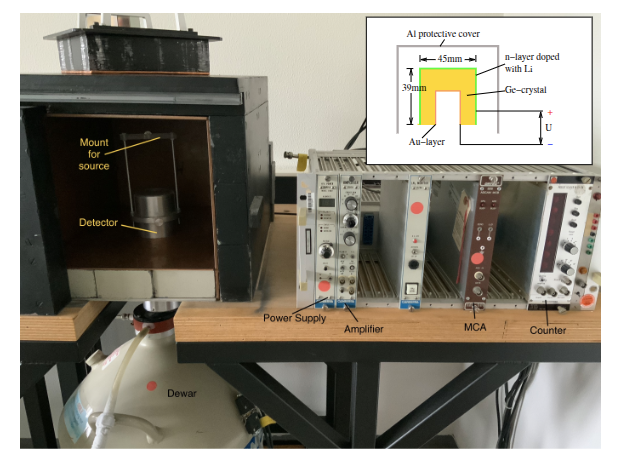
\includegraphics[width=0.8\textwidth]{content/pics/setup.png}
    \caption{Experimental setup and sketch of the germanium detector~\cite{Durchfuhrung}.}
    \label{fig:setup}
\end{figure}

The germanium detector  has a cylindrical shape and is protected by an outer $\mathrm{Al}$ layer. 
The crystal itself is also being coated from the outside with $\mathrm{Li}$ atoms with a width of $\qty{0.5}{cm}$ and from the inside with $\mathrm{Au}$ of a thickness of $\qty{20}{\micro\meter}$. 
Through that the $n$- and $p$-doping of the crystal is achieved, where $\mathrm{Li}$ is a donator ($n$-doping) and $\mathrm{Au}$ an acceptor ($p$-doping).
This is crucial for the effective detection of $\gamma$-photons, as described in~\autoref{sec:theory_detection} \textbf{REF ZU THEORY DETECTION}, but on the otherside has the effect that only photons whith energies above $40 - \qty{50}{\kilo\electronvolt}$ are being detected as others do not arrive at the germanium crystal.

\subsection{Procedure}


Before being able to measure the spectrum of several radioactive sources, the MCA was calibrated.
That was done using a $^{152}\mathrm{Eu}$-Source, that has several easily seperated photopeaks and hence the then experimentally observed channel numbers of those can be mapped with the source spectrum to get a function that allows to interpret channel numbers as desposited energy.
The $^{152}\mathrm{Eu}$-spectrum and all of the following spectra were measured for around one hour (with exact values following in~\autoref{sec:Analysis}).\\

Secondly a monochromatic $\gamma$-spectrum was measured, in order to observe the compton continuum, compton edge, backscattering peak and photopeak precisely.
For that a $^{137}\mathrm{Cs}$-emitter was used. \\

After that the spectrum of $^{133}\mathrm{Ba}$ was measured to determine the activity of the source, as well the spectrum of an unknown source to identify its content nuclides. \\

Finally, a background measurement without a source was done, in order to be able to remove the backgrund effect from the measurements before. 
For that measurement, a time greater than one hour was used. 

\clearpage